\section{Approach Designs}
In this section, we first introduce the background (\cref{sec:concepts}), then list the design requirements (\cref{sec:requirements}) and our system overview (\cref{sec:overview}).
% Lastly, we present a system overview that demonstrates our pipeline. (\cref{sec:overview}).


\subsection{Background and Concepts}
\label{sec:concepts}
% To aid the understanding of quantum terms and concepts, we have included a glossary in the supplementary materials.
\subsubsection{Quantum Circuit Model}
\label{sec:framework}
Analogous to classical circuits including bits and logic gates, quantum circuits are made up of qubits and quantum gates\cite{Nielsen:2010:QCBook}.
% A general quantum circuit consists of qubits, quantum gates, and measurements.

\textbf{Qubit.}
In quantum computation, quantum qubits, \emph{i.e.} qubits, are basic units of information storage.
A qubit is a ``quantum version'' of a classical bit.
Compared to the classical bit that can be either 0 or 1, a qubit can stay in a \emph{superposition} state\cite{Nielsen:2010:QCBook}.
Mathematically, a qubit state is represented as a linear combination of classical states $|\psi\rangle=\alpha|0\rangle + \beta|1\rangle$, where $|0\rangle$ and $|1\rangle$ represent the classical states 0 and 1, respectively.
Complex parameters $\alpha$ and $\beta$ can be configured via the quantum operation.

% the possible states of a qubit include $|0\rangle$ and $|1\rangle$, like the states 0 and 1 for a classical bit.


\textbf{Quantum gate.}
% In the procedure of quantum computation, the states of qubits are operated by quantum gates.
% The circuit starts with an initial state, which is typically a simple state like $|0\rangle$, and then the gates are applied one after another, transforming the state of the qubits in a specific way.
% For example, a X-gate would inverse the state of a qubit from $|0\rangle$ to $|1\rangle$, like a classical NOT-gate.
% And a CNOT-gate (Controlled-X gate) would inverse the state of a qubit depended on another qubit.
% As shown in {\cref{fig:qc-samples}-A2}, the state of ``q[1]'' is transformed following $|0\rangle \rightarrow |1\rangle \rightarrow |0\rangle$.
% There are various primitive gates used in quantum computing.
% In this research, these gates are unified into two distinct categories: \emph{single-qubit} gates (\emph{e.g.}, X-gate)  and \emph{multi-qubit} gates (\emph{e.g.}, CNOT-gate).
% As the name suggests, a single-qubit gate operates on one qubit at once, whereas a multi-qubit gate interconnects multiple qubits and perform operations on them simultaneously.
% The multi-qubit operations result in the \emph{entanglement} of qubits, which is a crucial factor of quantum advantage\cite{Jozsa:2003:REQ}.
% If two qubits are entangled, their states are logically related and cannot be described independently.
In a quantum circuit, operations on qubits are specified by quantum gates.
Given an initial state of multiple qubits, each gate of the circuit operates one or more qubits, which changes the parameters of qubits~(e,g, $\alpha$ and $\beta$).
For example, a Pauli-X-gate can invert the state of a qubit from $0|0\rangle + 1|1\rangle$ to $1|0\rangle + 0|1\rangle$.
There are many types of quantum gates~(e.g., X-gate and CNOT-gate) introduced in \cite{Nielsen:2010:QCBook}.
In summary, all gate types can be categorized into \textit{single-qubit gates} and \textit{multi-qubit gates}.
A single-qubit gate only operates one qubit, while a multi-qubit gate can operate more qubits, which creates entanglement between qubits~(correlations between parameters of different qubits).
Note that two quantum gates can be executed simultaneously in a circuit if they do not operate the same qubit, leading to parallelism in the qubit timelines.


% \textbf{Measurement.}
% To obtain the output of quantum computation, the quantum circuit is measured, which collapses the superposition of the qubits into a definite state. 
% The measurement result represents the output of computations.
% In general quantum programs, measurements are performed at the end, which do not correlate with the procedure of computations.
% Our research focuses on the representation and analysis of computation procedure that involves only qubits and quantum gates.

% \textbf{Gate composition.}
% Despite of the above primitives, some fixed compositions of quantum gates (\emph{e.g.}, data encoding modules\cite{Schuld:2019:QML, LaRose:2020:RDE}, quantum Fourier transform (QFT)\cite{Ruiz-Perez:2017:QFT}) are reused as components of quantum circuits,
% such as the ``adder'' is reused in the ``multiplier''.
% A functional composition of gates can be seen as a super-gate which has more complex functionality than individual primitive gates.
% In this paper, we refer the composite gates as \emph{component gate}, as opposed to the individual primitive gates.


\subsubsection{Visual Representation of Quantum Circuit}
% \st{To better understand the quantum circuit, a time-dependent diagram is widely adopted by quantum researchers to present its structure and procedure.
% As a common practice in quantum research, a time-dependent diagram is adopted to present the structure and procedure of a quantum circuit for better understanding.
% Our research is based on this general representation.}
% A typical quantum circuit diagram comprises the basic units outlined in the framework (\Cref{sec:framework}).
To interpret the quantum circuit, a time-dependent diagram is widely adopted.
The creation of a quantum circuit diagram involves both glyph representation and layout.
Here we briefly introduce these concepts.
% \hl{Drawing a typical quantum circuit diagram involves designing glyph and layout. Here we briefly introduce its typical visual encoding.}

\textbf{Basic glyphs.}
% \st{The elements of the quantum circuit (outlined in \cref{sec:framework}) are represented as primitive glyphs in the diagram.
% This paper presents them in a uniform visual representation as follows:}
% \hl{Both qubits and gates have visual representation in the circuit diagram:}.
The qubits and quantum gates are represented as glyphs in the diagram.
This paper presents them in a uniform visual representation as follows:
\begin{itemize}
    \item[\icon{qubit}]
     \emph{Qubit wire.}
      A qubit is represented as a horizontal wire in the diagram, %\hl{like storyline?}
      and a set of parallel qubit wires forms the basis of a quantum circuit diagram.

    \item[\icon{singlegate}]
     \emph{Single-qubit gate.}
     A single-qubit gate is represented as a square box placed on a qubit wire, which is labeled with the names of gates to differentiate between distinct types of gates, such as ``H'' for a Hadamard gate, ``X'' for a Pauli-X gate.
     % Examples of single-qubit gates include the Hadamard gate and the Pauli-X gate. 
    %   The blocks are labeled with the names of gates to differentiate between distinct types of gates, such as ``H'' for Hadamard gate and ``X'' for Pauli-X gate.
    
    \item[\icon{multigate}] \emph{Multi-qubit gate.}
      A multi-qubit gate is represented as boxes or dots on the qubit wires, which are vertically connected.
      % Additionally, the boxes and dots indicate different roles of the qubits~(target or controlled). 
      These boxes and dots also serve as an indication of the qubit's role as either a target or controlled qubit. 
      The boxes are also labeled to reflect the specific gate type, such as ``CX'' for a CNOT gate.
      % and horizontally laid on multiple qubit wires, which indicates the gate operates on all connected qubits.
      % An additional control wire with a dot end indicates the control qubit of the gate.
      % Examples of multi-qubit gates include the CNOT gate and the SWAP gate.
    %   The blocks are labeled with gate names as well.
    
    \item[\icon{component}] \emph{Component gate.}
    A component gate is a composition of multiple other gates.
    It is represented as a rectangular box spanning one or more qubit wires.
    The component gate is typically used to simplify the representation of more complex gates in the diagram.
    % For example, the QFT module is typically represented as a component gate composed of several single-qubit and multi-qubit gates in order to simplify its representation.
    % {\color{blue}Figure X} shows an component gate that performs the QFT operation on several qubits.
\end{itemize}
% The boxes of quantum gates are labeled with the names of gates to differentiate between distinct types of gates, such as ``H'' for Hadamard gate, ``X'' for Pauli-X gate, and ``CX'' for CNOT gate.


\textbf{Layout.}
% \st{On the basis of these glyphs, the layout of a quantum circuit diagram conveys specific meanings.
% It provides important visual cues to help readers understand the structure and operation of the circuit.
% For example, the vertical position of a gate on a qubit wire indicates the order in which gates are applied to a qubit, 
% while the horizontal placement of multi-qubit gates indicates the entanglement between qubits.
% In practice, various layout strategies are employed to emphasize specific aspects of the circuit or optimize for certain goals,
% such as minimizing the length of the circuit by positioning all gates to the left of idle wires
% or alleviating parallelism overload by shifting some gates to the right. This work adopts a semantic-preserving layout strategy in order to enhance the readability of the circuit diagram (\cref{sec:segment}).}
The layout provides important visual cues to help understand the circuit.
% For a gate, the notation type corresponds to its operation type.
% Its horizontal and vertical positions specify the operation order and operated qubits, respectively.
Each gate's notation type corresponds to its operation type, while its horizontal and vertical positions specify the order of operations and the qubits being operated upon, respectively.
Notations of multiple-qubit gates connect multiple qubits, indicating potential entanglement between qubits.
The layout can be modified to meet certain goals while keeping the circuit equivalence.
Specifically, the horizontal position of a gate can be moved forward or backward, as long as the order of gates on each qubit remains unchanged.
This work adopts a semantic-preserving layout strategy to enhance the readability of the circuit diagram (described in \cref{sec:segment}).

% Quantum gates are arranged on the qubit wires in the order that they are applied. 
% They are often arranged in a grid-like pattern, with each row representing a single qubit and each column representing a specific time step in the computation. 
% The resulting layout is often referred to as an orthogonal layout, which provides a clear and concise way to visualize the flow of operations in a quantum circuit.
% {\color{blue}+ explanation for placement adjustment.}
% All gates are laid on qubit wires in the sequence of computations.
% The gate layout is orthogonal including $n$ rows and $m$ columns,
% where $n$ equals the number of qubits, and $m$ is known as the length of the circuit.
% Each row contains exactly one qubit wire, and each column contains a list of gates that would be executed at the same time.
% One qubit is allowed to be operated by one gate at one time.

% \textbf{Alternative representations.}

% \textbf{Usage.}
% Quantum circuits are used in various stages of quantum computing workflow\cite{Weder:2020:IQC, Weder:2020:QSL}, including algorithm design, execution, analysis, and optimization.
% In the design process of quantum algorithms, the quantum circuit is a fundamental tool used to represent the computation.
% Researchers convey concepts and translate equation descriptions of the algorithm through the circuit.
% For example, {\Cref{fig:qc-samples}-C} illustrates a circuit representing quantum PCA algorithm\cite{Martin:2021:TPFD}.
% Once the quantum algorithm has been designed, the next step is implementation.
% The most common way to implement quantum algorithms is programming circuits using programming languages.
% The programming process involves translating quantum circuit diagrams to code statements and arranging quantum gates in a way that will solve the problem efficiently.
% After the program has been written, the next step is to optimize the quantum circuit to make it more efficient or to reduce errors.
% This can involve techniques such as gate synthesis, circuit transformation, and error correction.
% % The quantum circuit visualization plays an important role in this process.
% Finally, the quantum circuit is executed on a quantum computer or simulator to obtain the result of the computation. 
% The output of the circuit is typically probabilistic, meaning that it provides the probability of obtaining each possible output state. 
% The result is then post-processed to extract the relevant information from the output state.
% The complex nature of quantum mechanics and the non-intuitive behavior of quantum systems
% making the use of quantum circuits a unique and challenging area of study in quantum computing.
% However, existing visualization techniques are limited for scalable quantum circuits.
% {\color{blue}Need to shorten.}

\subsection{Design Requirements}
% \subsection{Design Requirements}
\label{sec:requirements}
The target users of this work are quantum researchers.
Two domain experts from university labs were involved in the entire process of this research.
In their daily work, quantum circuit diagrams are major visualization tools to interpret quantum circuits.
We conducted iterative interviews with them to distill requirements. 
They propose the requirements for large-scale quantum circuit analysis, which can be translated into visualization requirements below.

\textbf{R1. Clarify the components of quantum circuits.}
When designing quantum algorithms, it is common to use some typical sub-circuits as components of entire circuits.
Quantum researchers could easily recognize a typical component in an isolate circuit.
However, in a complex quantum circuit that consists of numerous quantum gates, it is challenging to identify and distinguish components from the general quantum circuit diagram.
Therefore, new diagrams should clarify the structure of quantum circuits with multiple components.

\textbf{R2. Simplify the patterns of quantum gates.}
Performing batch operations increases the scale of quantum circuits, and results in repeated patterns in circuit diagrams.
In practice, quantum researchers need to identify patterns in diagrams to understand the circuits.
Nevertheless, repeatedly examining patterns imposes a substantial cognitive load.
Therefore, new diagrams should reveal the patterns of quantum gates and reduce unnecessary repetitions.

\textbf{R3. Explicate the context of qubits and quantum gates.}
Quantum researchers have different concerns in quantum circuit analysis, such as qubit provenance\cite{Huang:2019:SAVA}, idling\cite{Das:2021:ADAPT}, quantum gate parallelisms\cite{Figgatt:2019:PEO} and the entanglement of quantum circuits\cite{Hubregtsen:2021:EPQC,JavadiAbhari:2014:ScaffCC}.
\added{These considerations are essential for programming and debugging circuits.
% However, they are implicit in exploring large circuit diagrams because the context of qubits and gates becomes complex and difficult to comprehend.
However, when exploring large circuit diagrams, these contextual details become intricate and challenging to comprehend.
% Therefore, new diagrams should explicate the context information to support idling, parallelism and entanglement analysis of quantum circuits.
Therefore, new diagrams should explicitly present context information, enabling the analysis of idling, parallelism, and entanglement in quantum circuits.}

\textbf{R4. Adopt familiar visual designs and flexible interactions.}
As our users are specialized in quantum computing, they have no experience in visual analysis. 
Thus, a concise and familiar design is preferred.
Also, they need flexibly-customized visualizations on demand.
For example, some users focus on the outline of the circuit, while other users are interested in details of qubits.
New diagrams should thus use visual designs that are intuitive and familiar to quantum researchers.
% , as well as easy to use and customize.

\subsection{System Overview}
\label{sec:overview}
To fulfill these requirements, we design {\tname}, a proof-of-concept system that visualizes scalable quantum circuits.
\Cref{fig:system-overview} illustrates the architecture of the system.
A novel visualization approach (\cref{sec:pipeline}) is undertaken.
It accepts a piece of quantum programming code, and generates flexibly-organized quantum circuit diagrams with comprehensive context information.
A user interface and a series of interactions (\cref{sec:system}) are provided to support interactive exploring and analysis of the quantum circuits.
\added{{\tname} is implemented as a Visual Studio Code plugin and available at \url{https://github.com/MeU1024/qc-vis}.}

\begin{figure}[htb]
    \centering
    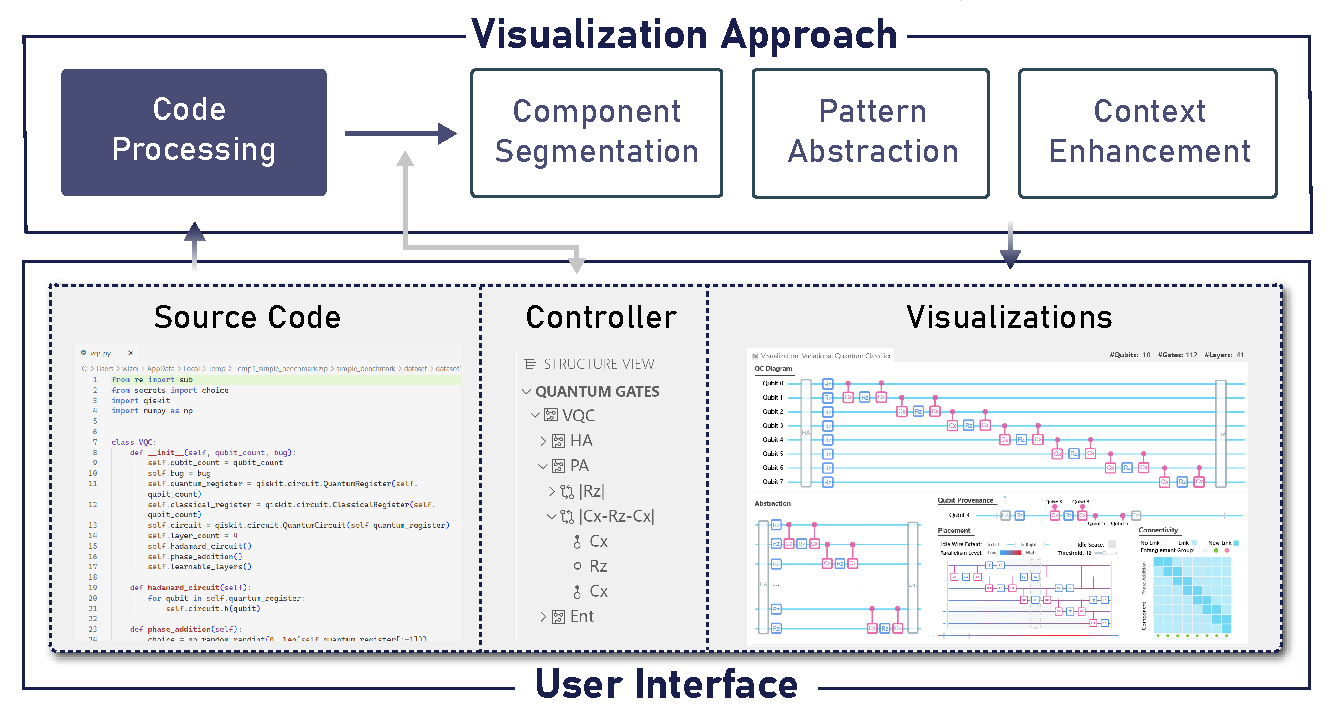
\includegraphics[width=\columnwidth]{system-overview}
    \caption{%
    System overview. {\tname} has a four-step visualization pipeline with a three-part interactive interface.%
    }
    \label{fig:system-overview}
\end{figure}

